\hypertarget{Approach}{
}

Our goal in this research is to investigate the usage of different reflection models for the generation of novel image data for material classification. For the image synthesis procedure of materials, we need the surface albedo and surface normals for every point of a material surface. In section \ref{sec:PhoTex}, the database used throughout this research is outlined. Due to the unavailability of the {\it ALOT} database at the time of this research, only the {\it PhoTex} database is considered for the experiments. The recovery of the surface albedo and surface normals from image data of a material can be done using photometric stereo. This method and its drawbacks will be outlined in section \ref{sec:SimplePhotometricStereo}. The remainder of this chapter discusses the classification method used (\ref{sec:Classification}) and how more complex reflection models can enhance the quality of synthetic image data (\ref{sec:ReflectionModels}).

\section{The PhoTex Database}\label{sec:PhoTex}
The PhoTex database is created for physics-based computer vision. It provides excellent image data for the recovery of surface albedo and surface normals, since all image data is created under controlled conditions. The materials are recorded under a fixed view and different illumination angles. It also provides the materials under a rotated angle, but these images are discarded for the experiments conducted in this research. The most important features of the database for this research are:

\begin{itemize}
	\item Images are gray scale
	\item For each image of a material class, every pixel in the image corresponds to the same point on the material surface
	\item The measured intensity in the images is proportional to irradiance
\end{itemize}

\noindent The database mainly holds images of rough surfaces, and a few smooth surfaces. For all the image data, the azimuth and zenith angles of the light source are provided (these angles are also mentioned as slant and tilt respectively), making it perfect for photometric stereo algorithms to recover the surface normals and surface albedo of the materials. The general setup for recording the materials can be seen in figure \ref{fig:PHOTEX_SETUP}. 

The example images are shown in figure \ref{fig:PhoTexExamples} --- these examples give an indication of how much the materials can vary in appearance when observed from different illumination angles.

In order to deal with possible illumination changes in both original and synthesized data, it is desirable to preprocess the images such that they are intensity invariant by setting the images to zero-mean and unit-variance before computing the image responses. 

\begin{figure}[htbp!]
	\begin{center}
		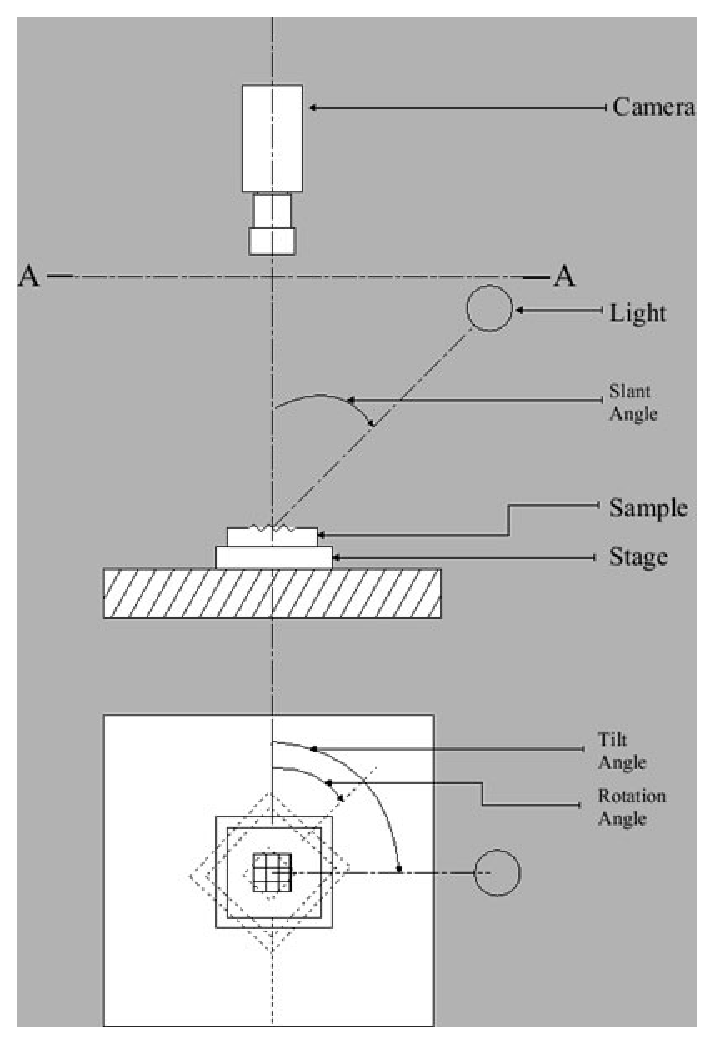
\epsfig{file=images/photex_setup.eps, width=0.5\linewidth}
	\end{center}
	\caption{{ \it Experimental setup of the recording of the PhoTex Database. Courtesy TextureLab @ Heriot-Watt University}}
	\label{fig:PHOTEX_SETUP}
\end{figure}

\section{Photometric Stereo}\label{sec:PhotometricStereo}
The aim of photometric stereo is to estimate at every point of a given object the surface albedo and surface normal. This is done by using a set of images of this object recorded under different illumination conditions. Different methods exist for photometric stereo that deal with different constraints and assumptions. There exist methods that use color information of the objects or use different colored light sources. However, since we deal with grayscale images from the {\it PhoTex} database, the photometric stereo method used in this research is restricted to grayscale images only.

\subsection{A Simple Photometric Stereo model}\label{sec:SimplePhotometricStereo}
Introduced by Woodham \cite{Woodham} in 1980, he devised a method to determine surface normals and the surface albedo from a set of images recorded under controlled conditions. The viewpoint is assumed to be orthogonal to the surface patch that needs to be recovered and on a fixed distance for all images. The source light illuminating the surface patch is assumed to be a point light --- the source is positioned at an infinite distance which as a result gives equal angles of incidence for all points on the surface patch. Using the assumption that the surface patch scatters light perfectly Lambertian and assuming there is no global illumination present in the data, the radiant exitance $B$ at a point $(x, y)$ on the surface can be written as:

	\begin{eqnarray*}
		B(x,y) = \rho(x,y)N(x,y) \cdot \mathcal{V}
	\end{eqnarray*}

\noindent Here, $\rho(x,y)$ is the surface albedo at point $(x,y)$, $N(x,y)$ is the surface normal at point $(x,y)$ and $\mathcal{V}$ is the source light vector. Both the surface normal and source light vector are unit in length. With the assumption that the camera response is linear to the surface radiant exitance, the value for a pixel at point $(x,y)$ in the image is equal to the radiant exitance at that point. The above equation can be written as:

	\begin{eqnarray*}
		I(x,y) =  \textbf{g}(x,y) \cdot \mathcal{V}
	\end{eqnarray*}

\noindent Where $\textbf{g}(x,y)$ is equal to $\rho(x,y)\textbf{N}(x,y)$ and describes the properties of the surface we want to recover. Given that $\mathcal{V}$ is known for the image data, with enough dot products between $\textbf{g}(x,y)$ and $\mathcal{V}$, the values for $\textbf{g}$ could be recovered. With known values for $\textbf{g}$, the albedo and surface normals in turn could be recovered.

If we have $n$ images all recorded under the same viewing angle with $n$ different light sources with known light source direction, we can construct a matrix where all values $V_i$ are stacked on each other:

	\begin{eqnarray*}
		\mathcal{V} = \begin{pmatrix} V_1^T \\ V_2^T \\ ... \\ V_n^T \end{pmatrix}
	\end{eqnarray*}

\noindent Then, for each image point in our set of image data, the intensity values are stacked into a vector:

	\begin{eqnarray*}
		\textbf{i}(x,y) = \begin{pmatrix} I_1(x,y) \\ I_2(x,y) \\ ... \\ I_n(x,y) \end{pmatrix}
	\end{eqnarray*}

\noindent With the above described vectors, we come to the linear system:

	\begin{eqnarray*}
		i(x,y) = \mathcal{V}\textbf{g}(x,y)
	\end{eqnarray*}

\noindent This is a linear system that can be solved for $\textbf{g}$ for each point on the surface to be recovered. To solve this system, a minimum of three images is required to get three equations per pixel.

Regions that lay completely in shadow could potentially pose problems when solving this system. It is of importance to rule out such regions in the computation, and this is possible by constructing a matrix $\Psi(x,y)$:

	\begin{eqnarray*}
		\Psi(x,y) = \begin{pmatrix} I_1(x,y) & ... & 0 & 0\\ 
									0 & I_2(x,y) & ... & 0\\ 
									0 & 0 & ... & I_n(x,y) \end{pmatrix}
	\end{eqnarray*}

\noindent Assuming there is no ambient illumination, a point in an image which is completely in shadows will give a 0 as a measurement. Multiplying both sides of the equation will rule out those points in the computation:

	\begin{eqnarray*}
		\Psi(x,y)\textbf{i} = \Psi(x,y)\mathcal{V}\textbf{g}(x,y)
	\end{eqnarray*}

\noindent Solving the above linear system for $\textbf{g}$ will make it possible to retrieve surface albedo and normals at each point $(x,y)$. Because the surface normal is unit in length, the surface albedo is $|\textbf{g}(x,y)| = \rho(x,y)$. The surface normal can be calculated as:

	\begin{eqnarray*}
		\textbf{N}(x,y) = \frac{1}{|\textbf{g}(x,y)|}\textbf{g}(x,y)
	\end{eqnarray*}


\subsection{Drawbacks}\label{drawbacks}
With the surface albedo and normals recovered, it is possible to synthesize images from the materials using reflection models. It is of importance to notice that this photometric stereo approach uses the Lambertian assumption to simplify the problem and this becomes a potential bottleneck. Since there are no such properties as specularity incorporated in the Lambertian model, speculars in the image data can be treated as diffuse reflections in the recovered surface albedo. This is clearly an issue when using the surface albedo for synthesis using reflection models other than Lambertian, since adding a specular on top of a retrieved specular could increase the error in image quality with respect to the original image.

To overcome this problem we tried various methods to decrease this error in the surface albedo (and consequently, surface normals). The first method is to use a {\it RANSAC} approach (RANdom SAmpling Concensus) to sample multiple surface albedo's of a point on the surface from the image data and compare them to detect outliers in the surface albedo. However, determining a threshold for outliers is difficult to find since different configurations of image data yield different errors and these thresholds are needed for each material independently. Also, it would make the comparison with Targhi's experiments difficult when using a minimal amount of training images for texture synthesis since there are only limited configurations possible when using 4 images, and none when using 3 images. 

Another way to overcome the problem is to construct the training sets in such way that the tilt angles are chosen uniform over the hemisphere. With this approach, the perfect configuration of data is used for photometric stereo, and outliers such as speculars in the surface albedo will have a small influence.

\section{Classification}\label{sec:Classification}

In this research, the classification method of Broadhurst is adapted as described in section \ref{sec:MGD}. This section explains in detail how models for materials will be constructed and how these are used for classification.

For each texture class, the maximum responses from the MR8 filter bank for each image are recorded to get rotationally invariant features. Before convolution, the images are preprocessed to have zero-mean and unit-variance to make the data intensity-invariant. The maximum responses are chosen by summing up the pixel values for each filter response and then select the orientation with the maximum response at each scale for both anisotropic filters, giving a total of 6 responses. The 2 isotropic filters give the remaining two responses, giving a total of 8 filter responses. See figure \ref{fig:MR} for the filters used to compute the responses.

To create marginals from these image responses, we make the assumption that the 8 distributions from the MR8 filter bank are mutually independent. The eight maximum responses are transformed into vectors with their response values sorted in descending order. Since we know the number of pixels is constant for the images, and the number of bins is defined, the number of pixel values stored in a bin is given by {\it numPixels} divided by {\it numBins}, rounded down. The eqi-count histograms are formed by storing the average pixel value for every set of pixels within the bin. Each image is now represented by 8 marginal histograms.

To create the multivariate Gaussian model for each material class, we estimate the joint intra-class variation of the marginal histograms. Joint marginal distributions are created by concatenating the marginals of each image, giving high-dimensional vectors. PCA is applied on the joint marginal distributions for each of the 8 feature specific distributions over all training images in a material class, resulting in 8 subspaces for projection per material model. For our experiments we use 13 eigencomponents.

For classification, a novel image is mapped onto the eight subspaces of each feature specific distribution for each of the material models. The total projection error for a class is computed by summing up the projection error of each feature specific distribution. The class with the lowest projection error is considered the class to which the novel image belongs to. 

\section{Reflection Models}\label{sec:ReflectionModels}
With the demand of data to improve models for material recognition, it is of interest to look in the direction of image synthesis for the automatic creation of novel data. In previous work on image synthesis, done by Targhi as described in section \ref{sec:Minimal}, the synthetic data is being created using the Lambertian reflection model. This model effectively implements self-shadows and diffuse reflection, but not specularity or back-scattering of light. In this research, the application of more complex reflection models for synthesis is studied. The reflection models can be put roughly into two categories --- models based on empirical observations, which are easy to use and have only few parameters to be set but defy basic laws in physics, and models with more physical backgrounds, which are mathematically more complex, but simulate light behavior more realistic. Some of both type of reflection models will be discussed in detail in the next chapters and are implemented for the experiments.

Since every reflection model depends on one or more parameters to be set, and these parameters are not given for the materials in the database, these parameters need to be estimated. This estimation procedure is outlined in section \ref{sec:ParameterSetting}.


